\documentclass[12pt]{article}
\usepackage[utf8]{inputenc}

%THIS IS WHERE ALL THE SYDE STUFF IS
\usepackage{sydestyle}

% Other imports go here
\usepackage{graphicx}
\graphicspath{{figures/}}
\usepackage{amsmath}
\usepackage{hyperref}
\hypersetup{
    colorlinks,
    citecolor=black,
    filecolor=black,
    linkcolor=black,
    urlcolor=black
}


\title{Homework 2}
\classname{SYDE 543}
\author{Karan Thukral, 20460691, 4A}
\date{October 5, 2016}
\supervisortext{Course Instructor: Professor Shi Cao}

% Content here
\begin{document}

	% Start with a title page!
	\makereporttitle

	% Make a table of contents.
	%\tableofcontents
	%\newpage

	% Couldn't figure out how to automate this, but leave this line in to restart page numbers at 1 and with arabic numbers.
	\startarabicpagenumbers
	
	\section{Signal Detection Task: X-Ray Diagnosis}
	For the purposes of this report, using X-Rays for diagnosis is an example of signal detection theory in the medical field. Currently speciliazed radiologists are responsible for taking x-rays and diagnosing based on them. An example x-ray showing a patient with lung cancer is shown in Figure \ref{lungcancer}. As it can be seen from the x-ray, the radiologist is expected to make a diagnosis on studying the result and using their experience to supliment their decision.
	
	\begin{figure}[!ht]
		\centering
		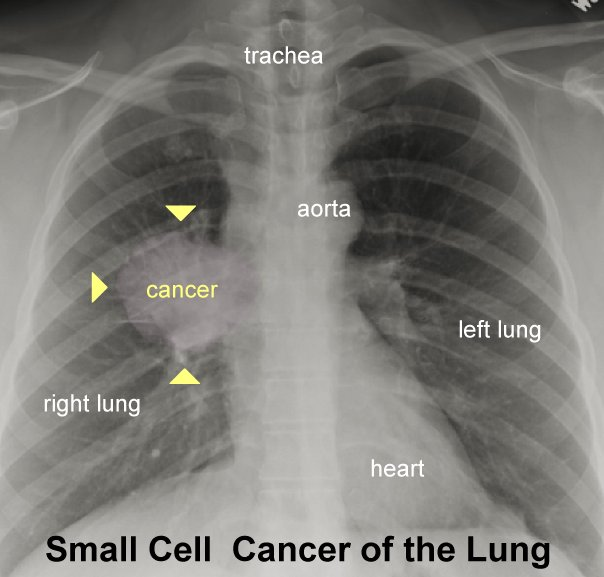
\includegraphics[width=0.5\textwidth]{lungcancer}
		\caption{Labeled X-Ray showing Lung Cancer}
		\label{lungcancer}
	\end{figure}
	
	\subsection{Signal Detection States}
	Based on a doctor's recomendation, a patient goes to a radiologist for an x-ray. The radiologist is responsible for using the result along with the doctors initial assesment to provide a preliminary diagnosis. This job can be stated as a signal detection problem as shown below. For the example case, we assume that the radiologist is looking for evidence of cancer.
	
	\begin{enumerate}
		\item *Hit*: The radiologist is correctly able to identify and diagnosis cancer using the x-ray
		\item *Miss*: The radiologist misses the evidence of cancer in the x-ray
		\item *False Alarm*: The radiologist diagnosis cancer when the patient does not have cancer
		\item *Correct Rejection**: The radiologist rejects cancer when the patient indeed does not have cancer.
	\end{enumerate}
	
	This leads to a generic signal detection problem where the radiologist response can either be a hit or a miss depending on their diagnosis and the true diagnosis about the patient.
	
	
	
	\subsection{Test Procedure}
	In order to test a radiologists capability to dishtinguish targets from non targets, the manager needs large amounts of patient x-rays whose diagnosis are already known. In order to measure the radiologists performance in regards to detecting cancer or not detecting cancer, the manager needs to measure their sensitivity. Sensitivity is the underlying ability to discriminate signals from noise. Figure \ref{sensitivity-graph1} shows graphs to illustarte the difference between noise and a signal. The x axis is the actual variable measured and the why axis is show the probability of x given that the measured variable is either noise or a signal.
	
	\begin{figure}[!ht]
		\centering
		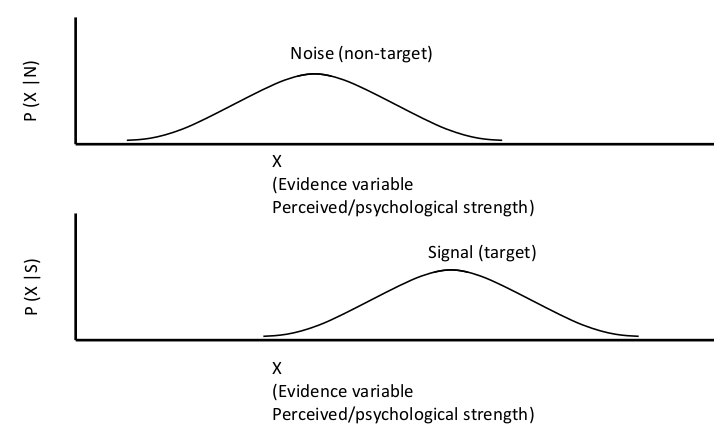
\includegraphics[width=0.5\textwidth]{sensitivity-graph1}
		\caption{$P(X|noise)$ and $P(X|signal)$. Noise = No cancer and Signal = cancer}
		\label{sensitivity-graph1}
	\end{figure}
	
	Due to the overlap in the signal and noise ditributions, the operator needs to develop a criterion $X_c$ such that the input if defined as noise ix $x\ <=\ X_c$ and signal otherwise. This is shown in Figure \ref{graph2}.
	
	\begin{figure}[!ht]
		\centering
		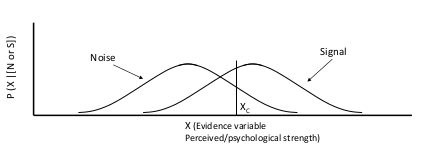
\includegraphics[width=0.5\textwidth]{graph2}
		\caption{}
		\label{graph2}
	\end{figure}
	
	A radiologist with betetr sensitivity has a much larger separation between the two distributions. A testing procedure along with all required calculations in explained below.
	
	\begin{itemize}
		\item Collect large amounts of known diagnosis along with x-rays
		\item Ask the radiologist to diagnosis the x-rays without informing them of the true diagnosis.
		\item Measure the number of time radiologist makes a correct diagnosis and everytime they make a wrong one.
		\item Use the number of correct diagnosis to calculate the probability of a hit and probability of correct rejections. $P(hit)=\frac{\text{number of correct cancer diagnosis}}{\text{total number of true cancer diagnosis}}$ and $P(correct\ rejection)=\frac{\text{number of correct non-cancer diagnosis}}{\text{total number of true non-cancer diagnosis}}$.
		\item Similarly calculate the probability of a false alarm and a miss. $P(false\ alarm)=\frac{\text{number of wrong cancer diagnosis}}{\text{total number of true non-cancer diagnosis}}$ and $P(miss)=\frac{\text{number of wrong non-cancer diagnosis}}{\text{total number of true cancer diagnosis}}$.
		\item With all the probabilities calculated, one can calculate the sensitivity ($d'$) of the radiologist. The ditributions shown in Figure \ref{sensitivity-graph1} are normal distributions. Thus to calculate $d'$, one needs the values of the probability constant ($Z$) from a table. $d'=Z(P(hit))-Z(P(false\ alarm))$.
	\end{itemize}	 
	
	With the value of sensitivity calculated above, the manager can make a sientific decision on the radiologist's performance. The larger the value of sensitivity, the better the radiologist is in differentiating between noise (no cancer) and signal (cancer).
	
	\subsection{Sensitivity Improvements}
	
	In order to improve the radiologist's senitivity, one first needs to increase their knowledge of the signal (cancerous x-ray). This can be done in the follwing ways,
	\begin{itemize}
		\item Providing example of the signal: This can be done by building a image recognition system to use the patient's x-ray and find similar diagnosed x-rays in order to provide some guidance to the radiologist. This can be done in a way to provide radiologists a second opinion without needing to find another specialist for it. Over time this second opinion will make their signal detection better.
		\item Regular tests: Radiologists should be made to reguarly go through a testing procedure like the one laid out above. This test is to provide the radiologists with more knowledge and common mistakes make by them. Having a consistent track of their sensitivity will make it easier for the radiologist to track their progress over time.
	\end{itemize}
	
	Another issue with the profession is the lack of resources when it comes to radiologists. Due to the low number of radiologists available, the rest are overworked and don't have the liberty of spending enough time studying the x-ray[]. In order to improve this from the manager's perspective, they need to limit the number of hours a radiologist is allowed to work. This aims to prevent fatigue and overload both of which can negatively affect the radiologist's senstitivity. This can be done by limiting over-time allowed or increasing the pay in order to attract more people to the profession. Another way for this would be to provide radiologists with breaks (apart from their lunch breaks) spread out throughout the day.
	
	\subsection{Response Criterion}
	In order to measure the radiologist's perference in the trade-off between more hits and avoiding false alarms, the manager needs to calculat their response criterion. In order to compute the decision criterion, the manager can use equation \ref{beta}. 
	\begin{equation}
		\beta = \frac{P(X|S)}{P(X|N)} = \frac{\text{Ordinate}(P(Hit))}{\text{Ordinate}(P(False\ Alarm))}
		\label{beta}
	\end{equation}
	
	$\beta$ is the ratio of signal probability density to noise probability density at $X_c$ which is the radiologists decision criterion. As $X_c$ moves left on graph as shown in Figure \ref{graph2}, $\beta$ decreaseas and the radiologists is more likely to detect a signal and vice versa in the other direction. A test plan is laid out below.
	
	\begin{enumerate}
		\item Collect large amounts of known diagnosis along with x-rays
		\item Ask the radiologist to diagnosis the x-rays without informing them of the true diagnosis.
		\item Measure the number of time radiologist makes a correct diagnosis and everytime they make a wrong one.
		\item Using the results from above to calulate the $P(hit)$, $P(false\ alarm)$ using the formulas provided above.
		\item Using the values calculated in the above step, find the ordinate values for $O(P(hit))$ and $O(P(false\ alram))$ using a constant table.
		\item With the ordinate values, calculate $\beta = \frac{O(P(hit))}{O(P(false\ alarm))}$
		\item Larger the $\beta$ value the more conservative the radiologist and vice versa.
	\end{enumerate}
	
	In order to calculate the optimal decision criteria, one needs to know the values (V) and cost (C) associated with a hit, miss, correct rejection and a false alarm along with $P(noise) = P(\text{no cancer x-ray})$ and $P(signal) = P(\text{cancer x-ray})$. For the purposes of this report, it is assumed that these values are known. The formula for the optimal decision criterion is shown in Equation \ref{beta-o}.
	
	\begin{equation}
		\beta_{opt} = \frac{P(\text{noise})}{P(\text{signal})} * \frac{[V(\text{correct rejection}) + c(\text{false alarm})]}{V(\text{hit}) + C(\text{miss})}
		\label{beta-o}
	\end{equation}
	
	\subsection{Decision Criterion Improvements}
	In order to allow radiologists to make better trade offs the following steps can be followed:
	
	\begin{enumerate}
		\item The main step to follow is to teach the radiologists about the value and cost associated with each of the options. If the radiologists know of a numeric value associated with the value of a correct rejection and cost of a false alarm, they will be able to make better decisons. Increasing this V(correct rejection) and C(false alarm) will increase $\beta$ leading to more conservative responses from the radiologists. This can be done through repeated training and having numeric values assigned to value and cost of each of the options.
		\item Another way to affect the radiologists decision criterion is to change the preceived signal and noise probabilities. This can be done by adding known x-rays with or without cancer dueing training and changing the number of these x-rays will cause a shift in $P(signal)=P(cancer)$ and $P(noise)=P(not\ cancer)$. Increasing $P(noise)$ will cause $\beta$ to increase leading to a more conservative behaviour whereas increasing $P(signal)$ will decrease $\beta$ and lead to more risky (say "yes" more) behaviour.
		\item The last way to improve this would be to teach the radiologists using existing/past known cases and disussing the results of the diagnosis made. As an example, studying a case where a radiologist missed a cancer diagnosis and the result will make help adapt the radiologists percieved payoffs of outcomes. Similarly studying the negative effects of a false alarm in a past case will make them be more cautious. Selecting these known cases and using them can help change the perceptions of radiologists and help get them to conform to a desired response criterion.
	\end{enumerate}
	
	
\end{document}
